\section{Merging L1 and L2}

\begin{frame}{Burst time and duty-cycle}{}
	\begin{block}{Only 3-9 sec. burst and long break}
		Duty cycle: $T_{Burst}/ T_{Break} \approx 0.3$
	\end{block}

	\vspace{1cm}
	\begin{figure}[htp]
		\begin{center}
		  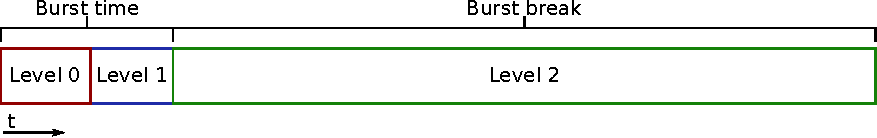
\includegraphics[width=\textwidth]{bursttime}
		  \caption{NA48 approach}
		\end{center}
	\end{figure}
\end{frame}

\subsection{New farm design}
\begin{frame}{Reuse L1 PCs}{}
	\begin{block}{My proposal to use resources more efficiently}
		Reuse L1 PCs during burst break for L2 computation by combining L1 and L2 to
		one farm
	\end{block}

	\vspace{1cm}
	\begin{figure}[htp]
		\begin{center}
		 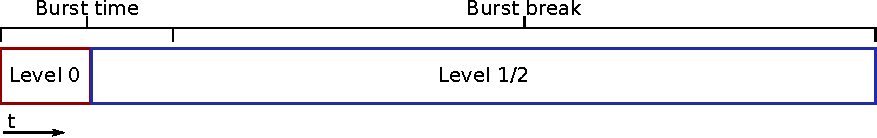
\includegraphics[width=\textwidth]{bursttime-l12merged}
		  \caption{New proposal}
		\end{center}
	\end{figure}
\end{frame}

\begin{frame}{Don't separate L1 and L2!}{}
	\begin{center} 
		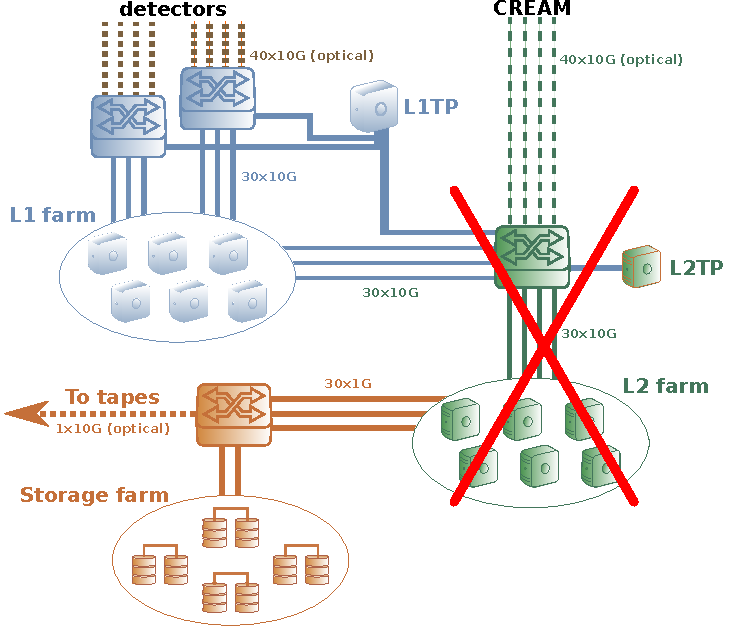
\includegraphics[width=0.8\textwidth]{whole-farm-nol2}
	\end{center} 
\end{frame}

\begin{frame}{Combine L1 and L2 to one farm}{}
	\begin{center} 
		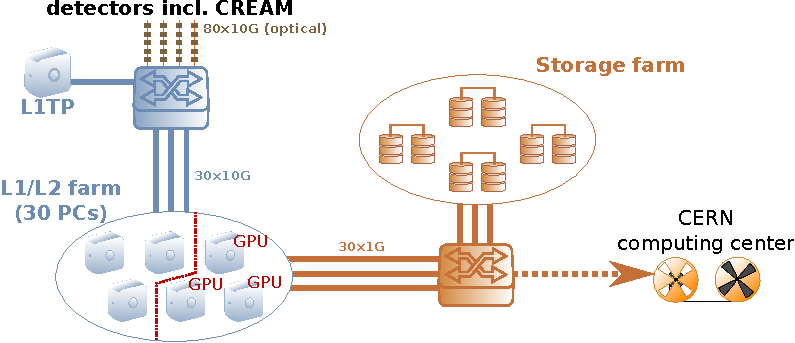
\includegraphics[width=0.9\textwidth]{merged-star}
	\end{center} 
	\begin{exampleblock}{We safe about 80k€}
		\begin{itemize}
		  \item No L1 PCs anymore
		  \item Less switches, less network cards
		\end{itemize}
	\end{exampleblock}
\end{frame}

\begin{frame}{New bottleneck}{}
	\begin{center} 
		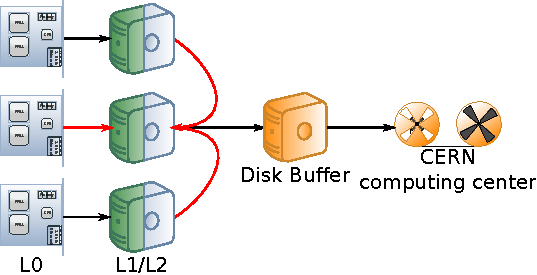
\includegraphics[width=0.6\textwidth]{dataflow-alert.pdf}
	\end{center} 
	
	\begin{alertblock}{Risk of overloading the farm (L1 and L2 concurrently)}
		Possibilities to solve this problem:
		\begin{itemize}
		  	\item Implement a very intelligent load balancing algorithm 
  			\item Wait with L2 until end of Burst (L1 has finished)
		\end{itemize}
	\end{alertblock}
\end{frame}

\subsection{Event building @ L1}
\begin{frame}{New proposal}{Event building @ L1}
	\begin{center} 
		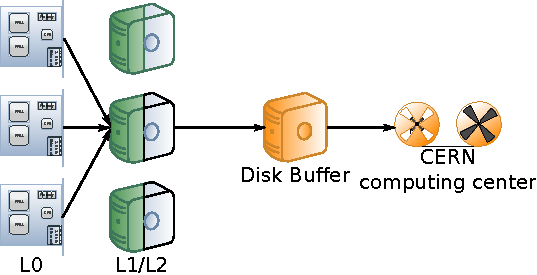
\includegraphics[width=0.6\textwidth]{dataflow-merged-gian}
	\end{center} 
	
	\begin{block}{Every subdetector sends data of an event to one single PC}
		\begin{itemize}
		  	\pro No broadcast of a L1 decision needed anymore (no L1TP)
		  	\pro Easier to implement load balancing (self-sustaining PCs)
  			\contra Every farm PC must serve every subdetector $\Rightarrow$ needs GPUs
		\end{itemize}
	\end{block}
\end{frame}

\begin{frame}{UDP Storm}{Congestion at one single farm PC}
\begin{columns}
	 	\column{.5\textwidth}
			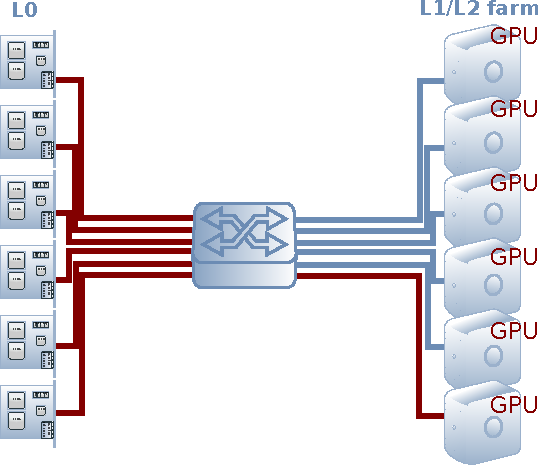
\includegraphics[width=\textwidth]{gianluca-congestion}
	    \column{.6 \textwidth}
	    	\begin{block}{Bundle events for better performance}
	    		Smallest Event: 160 B \\
	    		Jumbo ethernet frame: 9 kB \\
	    		55 Events in one bundle \\
				$\Rightarrow$ $55\cdot5kB=275 kB$ total per bundle	    		
			\end{block}
			\begin{block}{Round Robin tables at L0}
				Send events 1-55 to PC A \\
				Send events 56-110 to PC B \\
				\ldots
			\end{block}
	\end{columns}
\end{frame}

\begin{frame}{Packet loss}{22 L0 boards simulated}
	\begin{center} 
		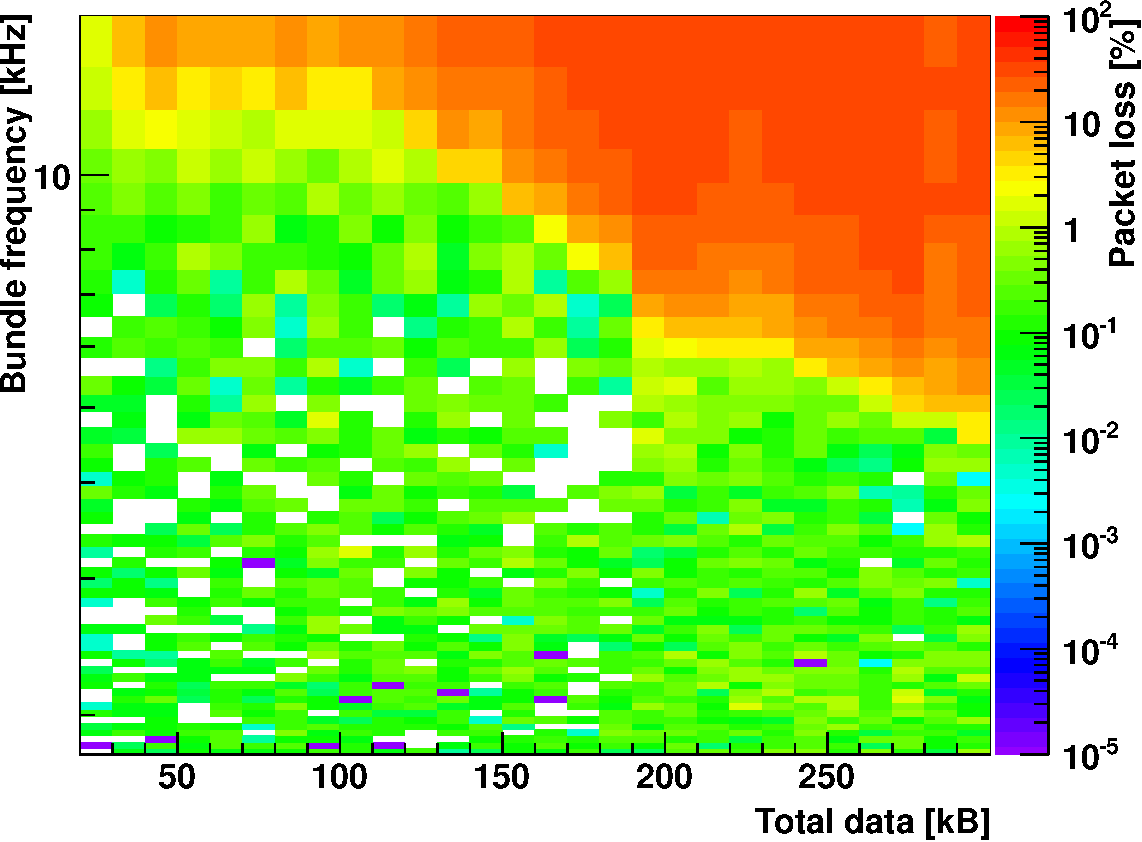
\includegraphics[width=0.9\textwidth]{udp-storm-packloss}
	\end{center} 
\end{frame}

\begin{frame}{Packet loss}{Under construction}
	\begin{block}{High packet loss}
		Packets are rejected by Kernel at receiver side (Not at switch or network
		card)!
		\\
		I'm investigating if we can use standard drivers or have to implement own
		ones
	\end{block}
	
	\begin{exampleblock}{Packets get lost in software, not hardware!}
		$\Rightarrow$ UDP storms don't cause problems \\
		
		Events can be merged at L1 which makes load balancing much easier (no L1TP
		needed)
	\end{exampleblock}
\end{frame}

\begin{frame}{No expensive core switch needed}{}
	\begin{block}{One expensive core switch was originally planned}
		\begin{itemize}
		  \pro Many ports (high density)
		  \pro Fast backplane (any to any @ 10Gbps bidirectional)
		  \contra High cost (about 180k€)
		\end{itemize}
	\end{block}
	\begin{block}{Tree topology with cheap 24 and 48 port switches}
		\begin{itemize}
		  \contra Slow backplanes (any to any @ 10Gbps only unidirectional)
		  \contra Bottleneck at switch-to-switch connection
		  \pro Low cost (about 80k€)
		\end{itemize}
	\end{block}
	\begin{exampleblock}{Only one way transmission with about 8Gbps per link}
		It is feasible to use slower switches
	\end{exampleblock}
\end{frame}

\begin{frame}{Tree topology (Hexapus)}{}
	\begin{center} 
		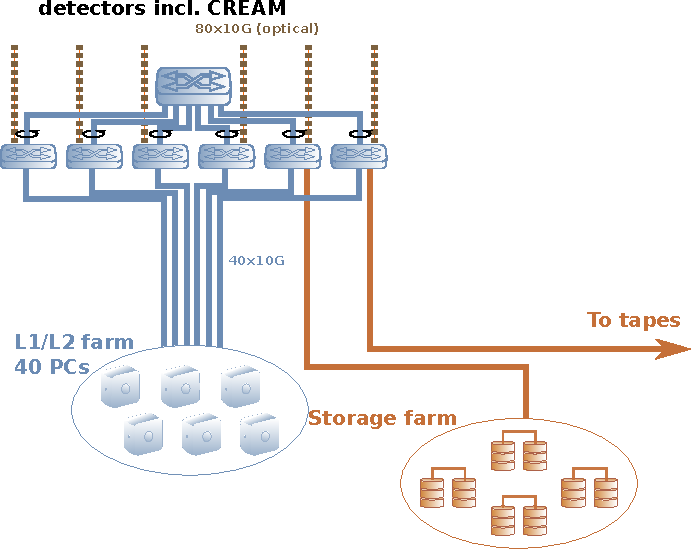
\includegraphics[width=0.9\textwidth]{whole-farm-l12merged-tree}
	\end{center} 
\end{frame}
